\section{Оборудование}
Переменное магнитное поле создается с помощью соленоида 1, намотанного на цилиндрический каркас 2 из поливинилхлорида, который подключается к генератору сигналов ЗГ (канал А).
Внутри каркаса расположен медный экран 3 в виде полого цилиндра.

Действующее значение переменного тока в цепи соленоида измеряется цифровым амперметром А
Действующее значение переменного напряжения на измерительной катушке 4  измеряется цифровым вольтметром V.

Для измерения сдвига фаз между током в цепи соленоида и напряжением на измерительной катушке используется двухканальный осциллограф.
На канал Y  осциллографа подается напряжение с измерительной катушки, а на канал X~--- напряжение с резистора R, которое пропорционально току в цепи соленоида.

Для другой схемы RLC-метр, измеряющий индуктивность,
подключается к катушке 1 через клеммы 5 и 6 на панеле установки. Другие приборы при
этом должны быть отсоединены от цепи, т.к. RLC-метр измеряет индуктивность активным
образом.

\begin{figure}[ht!]
    \center{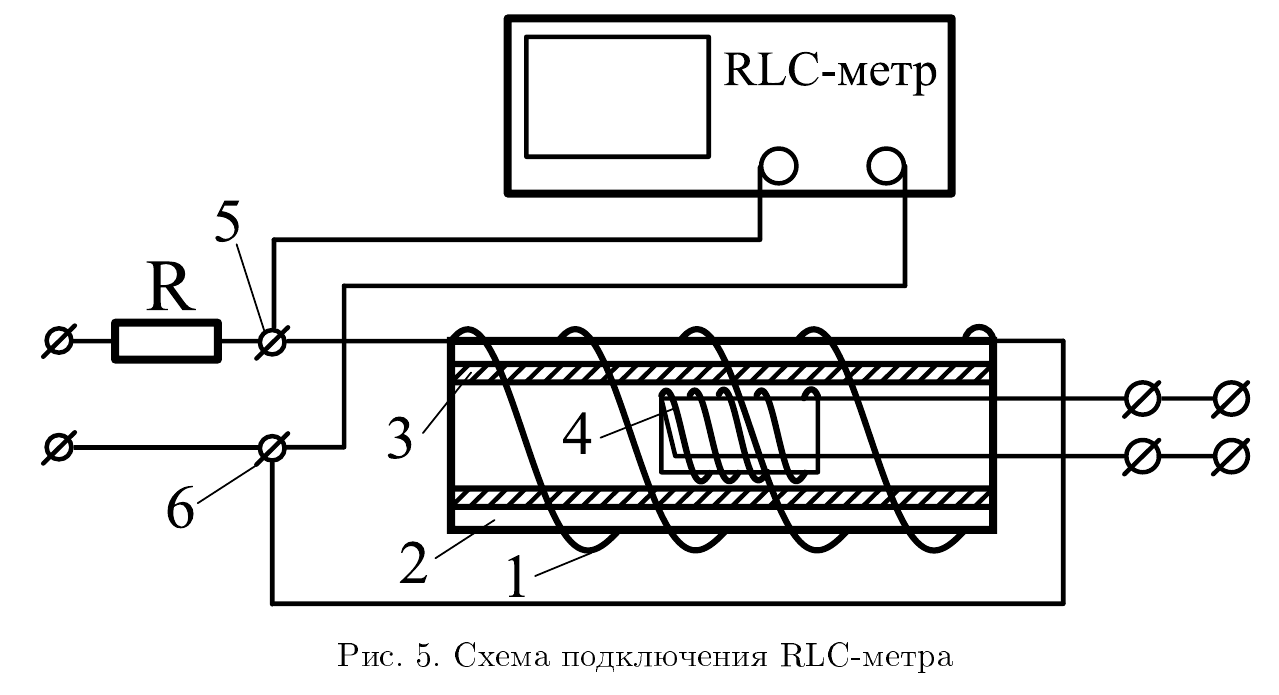
\includegraphics[width=0.8\linewidth]{../img/fig5.png}}
\end{figure}

\subsection{Измерение отношения амплитуд магнитного поля внутри и вне экрана}
С помощью вольтметра V измеряется действующее значение ЭДС индукции, которая
возникает в измерительной катушке, находящейся в переменном магнитном поле
$H_{1}e^{iwt}$. Комплексная амплитуда ЭДС индукции в измерительной катушке равна
\[
U = -SN\frac{dB_{1}(t)}{dt} = -iw\mu_{0}SNH_{1}e^{iwt}
\]
Показания вольтметра, измеряющего это напряжение:
\[
    U=\frac{SNw}{\sqrt{2}}\mu_{0}H_{1}
\]
\[
    H_{1} ~ U/\nu
\]
\[
    H_{0} ~ I
\]
\[
    \frac{H_{1}}{H_{0}} = \text{const}\cdot \frac{U}{\nu I}
\]
Таким образом, отношение амплитуд магнитных полей снаружи и вне экрана
может быть измерено по отношению $U/\nu I$ при разных частотах.
При низких частотах
\[
    \frac{H_{1}}{H_{0}}\to 1
\]

\subsection{Определение проводимости материала экрана по фазовому сдвигу}
В установке в качестве экрана используется медная труба промышленного производства.
Технология изготовления труб оказывает заметное влияние на электропроводимость.
Из-за наличия примесей проводимость меди нашей трубы отличается от табличного значения
в меньшую сторону. Для определения $\sigma$ предлагается использовать частотную зависимость
 фазового сдвига между магнитными полями внутри и вне
 экрана при низких частотах и зависимость при высоких частотах.

 $\tg\psi(\nu)$~--- линейная зависимость, проходящая через 0 (для низких частот).
 Для высоких частот такой зависимостью аппроксимируется $\psi(\sqrt{\nu})-\pi/4$.

 На входной канал Y осциллографа подаётся сигнал с измерительной катушки, который пропорционален не полю внутри экрана,
 а его производной по времени, а это означает, что появляется дополнительный сдвиг по фазе на
 $\pi/2$. Поэтому
 \[
     \varphi = \psi + \pi/2
 \]
 
 \subsection{Влияние скин-эффекта на индуктивность катушки}
 Из-за скин эффекта индуктивность соленоида с медным цилиндрическим экраном
 внутри будет зависеть от частоты тока. На высоких частотах магнитное поле не проникает внутрь соленоида (за экран), поэтому суммарный магнитный поток, пронизывающий
 катушку, уменьшается, и, соответственно, уменьшается и индуктивность. При низких частотах, когда толщина скин-слоя
 $\delta$ больше толщины медного экрана $h$,  магнитное поле
 проникает внутрь катушки, однако его амплитуда падает  и возникает
 разность фаз между колебаниями поля за экраном и перед ним.  Из-за
 чего также изменяется магнитный поток, а следовательно~--- и индуктивность.

 Рассмотрим магнитный поток через катушку как сумму двух магнитных потоков:
 пронизывающий область между катушкой и цилиндрическим экраном $\Phi_{out}$ и пронизывающий область за экраном $\Phi_{in}$.
 \[
     \Phi = \Phi_{out} + \Phi_{in} = H_{0}S_{0} + H_{1}S_{1} = LI
 \]
 $H_{0}$ и $H_{1}$~---  мгновенные значения магнитного поля внутри и снаружи цилиндра при
 данном токе $I$, $S_{0}$ и $S_{1}$~--- площади внешней и внутренней (по отношению к цилиндрическому
 экрану) областей соответственно.

 Очевидно, что минимальная индуктивность будет в случае, когда $\Phi_{in} = 0$.
 \[
     L_{min} = \frac{\Phi_{out}}{I}
 \]
 \[
     \Phi_{in} = H_{1}S_{1} = \frac{H_{1}S_{1}}{H_{0}S_{0}} \Phi_{out} = \frac{\Phi_{out}}{n}\frac{S_{1}}{S_{0}}
 \]
 \[
     n = \frac{H_{0}}{H_{1}}\frac{1}{\cos\psi}
 \]
 \[
     \Phi_{max} = \Phi_{out} + \Phi_{in_{max}} = H_{0}\left(S_{0}+S_{1}\right)=L_{max}I_{m}
 \]
 \[
     \frac{S_{1}}{S_{0}} = \frac{L_{max} - L_{min}}{L_{min}}
 \]
\[
    L = L_{min} + \frac{L_{max} - L_{min}}{n}
\]
\[
    \frac{L_{max} - L}{L - L_{min}} = \left(\pi a h \mu_{0} \sigma \nu\right)^{2}
\]
По углу наклона прямой можно определить $\sigma$. 
